\documentclass[a4paper]{article}
\usepackage{graphicx} % Required for inserting images
\usepackage{indentfirst}
\usepackage[brazil]{babel}
\usepackage{amssymb}
\usepackage{amsmath}
\usepackage{dsfont}
\usepackage[left=2.5cm,top=2.5cm,right=2.5cm,bottom=2.5cm]{geometry}
\usepackage{tikz}
\usepackage{float}
\usepackage{multirow}
\graphicspath{ {./images/} }

\title{Aproximação de modelos estatísticos não-uniformes por meio de MCMC - MAP2212}
\author{Antonio Gabriel Freitas da Silva - 13687290 \and Guilherme Vaz das Neves Hummel -  13733732 \and Marco Antonio Soares de Campos -  13686469}
\date{Maio 2023}

\begin{document}

\maketitle

\section{Introdução} 

O cálculo exato de distribuições "a posteriori" pode ser um processo impossível em diversos casos, as cadeias de Markov associadas aos Métodos Monte Carlo possibilitam a geração de valores por um longo período de tempo até que haja uma convergência para a sua distribuição estacionária, de tal forma que seus resultados possam estar seja gerada pela cadeia, existem alguns métodos para o uso desta ferramenta. Neste exercício-programa, será usado o algoritmo de Metropolis-Hastings, por superioridade em sua eficiência e alta dimensionalidade em quaisquer cirscunstâncias, além de demonstrar a sua capacidade de se adequar a variados problemas computacionais.  

\section{O algoritmo de Metropolis-Hastings}

O algoritmo de Metropolis-Hastings se apropria do uso de cadeias de Markov utilizando o seguinte roteiro:

\begin{enumerate}
    \item Amostrar uma função de probabilidade $f$;
    \item A cada amostragem, será realizada um salto/mudança aleatória, gerado por uma distribuição de transição, que neste caso será uma normal multivariada de média 0 e variância $\Sigma$;
    \item Teremos uma probabilidade de aceitação dada como $\alpha(i, j) = \frac{g(\theta^*)}{g(\theta_0)}$, levando em consideração os parâmetros da distribuição de transição escolhida.
    \item Compara-se a razão com um valor $x \in (0, 1)$, caso $x > \alpha(i, j)$, rejeita-se a proposta, caso contrário, aceita-se o valor.
    \item Dessa forma, será gerado uma sequência de valores aleatórios em Cadeias de Markov dados como $  \left\{  x_n \right\} $, que irão convergir de acordo com a distribuição dada.
    
\end{enumerate}
    
    Uma característica importante do algoritmo de Metropolis-Hastings é que ele permite a exploração de regiões de alta densidade da distribuição alvo, mesmo quando essas regiões são de pequena probabilidade. Isso é possível porque as amostras aceitas são ponderadas pela razão de aceitação, permitindo que as regiões de maior densidade sejam amostradas com maior frequência.

    No entanto, é importante observar que a eficiência do algoritmo pode depender da escolha adequada da distribuição de transição, pois essa escolha afeta a taxa de aceitação das propostas de salto. Além disso, o algoritmo pode exigir um tempo considerável para a cadeia de Markov atingir a distribuição estacionária e apresentar autocorrelações entre as amostras. Neste trabalho, o tempo de execução do programa está em cerca de 15min, a depender da sua taxa de aceitação.

    A variãncia da Normal Multivariada possui a seguinte relação:

    \begin{equation*}
    \begin{center}
        
    

        $\Sigma \propto (1-\lambda)S + \lambda D$

    \end{center}
    \end{equation*}

Sendo S uma matriz de covariância que é atualizada constantemente, D uma matriz diagonal para estimar inicialmente as variâncias marginais e $\lambda$ uma constante que é ajustada interativamente para se obter uma taxa de aceitação dos valores de $\alpha$ que são testados.

\section{Funções utilizadas}

Queremos calcular a função definida por $W(v)$ aproximada por uma função condensada de massa de probabilidade $U(v)$, sendo aquela dada como:

\begin{equation}
\begin{center}
    

$W(v) = \int_{T(v)} f(\theta | x, y) d\theta$

\end{center} 
\end{equation}

Além disso, o domínio da função será dada por um vetor definido por:

\begin{equation}
\begin{center}

$T(v) = \left\{ \theta \in \Theta \,|\, f(\theta | x, y) \le v \right\} $

\end{center}
\end{equation}

A função $f(\theta | x, y)$, por fins práticos, é definida por uma função de Dirichlet de parâmetros $x, y$ e $\theta$ dados por:

\begin{equation}
\begin{center}
    

$f(\theta | x, y) = \frac{1}{B(x + y)} \prod_{i = 1}^m \theta_i^{x_i + y_i -1 }$

\end{center} 
\end{equation}

Sendo B uma distribuição Beta e $x, y \in \aleph^m, \theta \in \Theta = S_m = \left\{ \theta \in \Re_{m}^{+} \, 
| f(\theta | x, y) \le v \,\right\}$, e $\theta$ um vetor de probabilidades que neste trabalho terá uma dimensão definida por $m = 3$, ou seja, um formato simplex.

\section{Amostragem desejada e cálculo do número de bins}

Foi utilizada uma aproximação assintótica através de uma distribuição Bernoulli com variância máxima de $0.25$ e sua normalização em $95\%$ de confiança e um erro $\varepsilon = 0.05\%$, a quatidade de bins será dada a partir de $k$, que reduz o erro que será parametrizado como:

\begin{equation}
\begin{center}
    

$W(v_j) - W(v_{j-1}) \approx \frac{1}{k} \le \varepsilon$

\end{center} 
\end{equation}

E pelo resultado do Teorema Central do Limite, teremos que:

\begin{equation}
\begin{center}
    

$n = (\frac{\sigma\cdot Z_{\alpha/2}}{\varepsilon})^2$

\end{center} 
\end{equation}

Dados que $\sigma^2 = 0.25$, $Z_{\alpha/2} = 1.96$ para a nossa amostragem geral, que torna:

\begin{center}
    

$n = \frac{3.8416 \cdot 0.25}{0.0005^2} = 3.841.600$

\end{center} 

Logo, precisamos de 3.841.600 de pontos para conseguirmos a precisão desejada.

Ao considerarmos apenas a igualdade, o cálculo dos bins foi feito da seguinte forma:

\begin{center}
    

$\frac{1}{k} = \varepsilon \implies k = \frac{1}{\varepsilon} \implies k = 2000$

\end{center} 

Nós utilizaremos o valor mínimo de bins (2000) para realizarmos a simulação.

\section{Simulação e conclusão}

A príncipio, o programa realiza o cálculo de v, que recebe um valor qualquer que retornará a sua acumulada, o cálculo de T, para avaliar o domínio que haverá através da distribuição de pontos através do algoritmo que mencionamos em capítulos anteriores divididos por uma constante de normalização dado como uma gamma dos valores $x, y$ distribuídos, depois calcula as acumuladas em seus bins respectivos. Dessa forma, progressivamente há avanço de passos que aumentam o valor da acumulada (U(v) no caso) até se tornar 1. Os valores das constantes e da taxa de rejeição são proporcionais neste caso.

\begin{figure}[H]
  \centering
  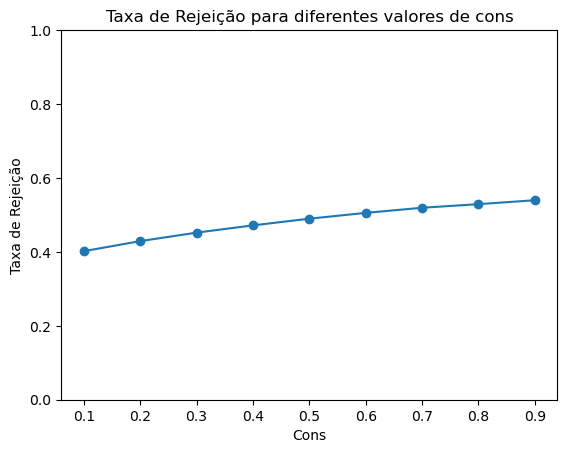
\includegraphics[width=0.5\textwidth]{Reject.png}
  \caption{Comparação entre a taxa de rejeição e a constante \lambda}
  \label{fig:HxU}
\end{figure}


\begin{table}[h]
\centering
\begin{tabular}{|c|c|c|c|c|c|}
\hline
v & U(v)  \\
\hline
0.5066 & 0.0163 \\
\hline
2.5 & 0.1058 \\
\hline
10.0 & 0.5528 \\
\hline
16.7 & 1.0 \\
\hline
\end{tabular}
\caption{Tabela de resultados dos métodos de integração, com seed de 39}
\label{tab:resultados}
\end{table}

O máximo desta função nos vetores mencionados na tabela será de aproximadamente $16.608$ (a "altura" da função em $\mathbb{R}^3$).

\begin{figure}[H]
  \centering
  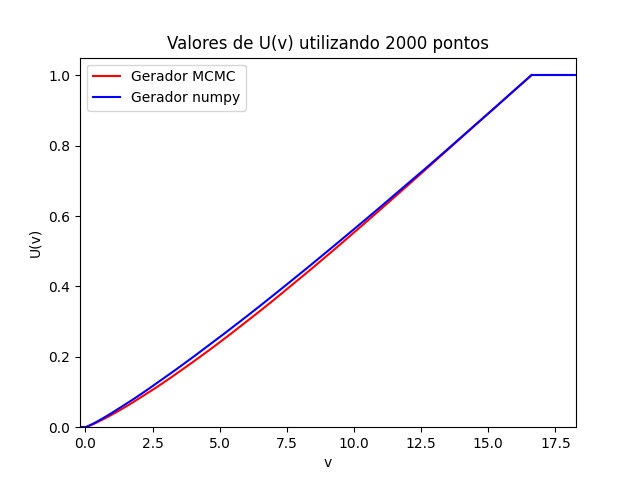
\includegraphics[width=0.5\textwidth]{Geradores.png}
  \caption{Gráfico de comparação entre a MCMC e Dirichlet}
  \label{fig:HxU}
\end{figure}

Comparadas ao método anterior, a distribuição se torna mais discrepante em seus resultados no início, logo, dessa forma, percebemos uma grande aproximação dos valores descritos, obtidos, no entanto, em um tempo de execução maior do que em seu anterior.

Portanto, temos que há uma verdadeira aproximação entre os métodos MCMC e da própria distribuição de Dirichlet, no entanto, o método das Cadeias de Markov demanda-se um tempo maior de execução.

\end{document}
